\documentclass[addpoints]{exam}
\usepackage[utf8]{inputenc}
\usepackage[portuguese]{babel}
\usepackage[LGRgreek]{mathastext}
\usepackage{graphicx,graphics}

\footer{}{\thepage}{}
 
\pointpoints{ponto}{pontos}
\bonuspointpoints{ponto extra}{pontos extra}
 
\totalformat{Pregunta \thequestion: \totalpoints pontos}
 
\chqword{Pregunta}
\chpgword{Página}
\chpword{Pontos}
\chbpword{Pontos extra}
\chsword{Pontos obtidos}
\chtword{Total}

\hqword{Questão}
\hpgword{Página}
\hpword{Pontos}
\hsword{Pontos obtidos}
\htword{Total}

 
\begin{document}
 
\begin{center}
Eletrônica Básica II – EE640 U - Lista de Exercícios 3
\end{center}
 
\vspace{5mm}
 
\makebox[0.72\textwidth]{Nome: \enspace\hrulefill}
\hfill
\makebox[0.2\textwidth]{RA: \enspace\hrulefill}

\begin{center}
A lista deve ser entregue até dia \textbf{01-01-1968}
\end{center}

\hspace{2mm}

\begin{center}
\gradetable[h][questions]
\end{center}

\hspace{2mm}

\begin{questions}

\question Dada a curva de transferência de malha aberta, determine:

\begin{parts}
 \part A função de transferência de módulo e fase;
 \part O valor mínimo de $\beta$ para o sistema ser estável
\end{parts}

\begin{center}
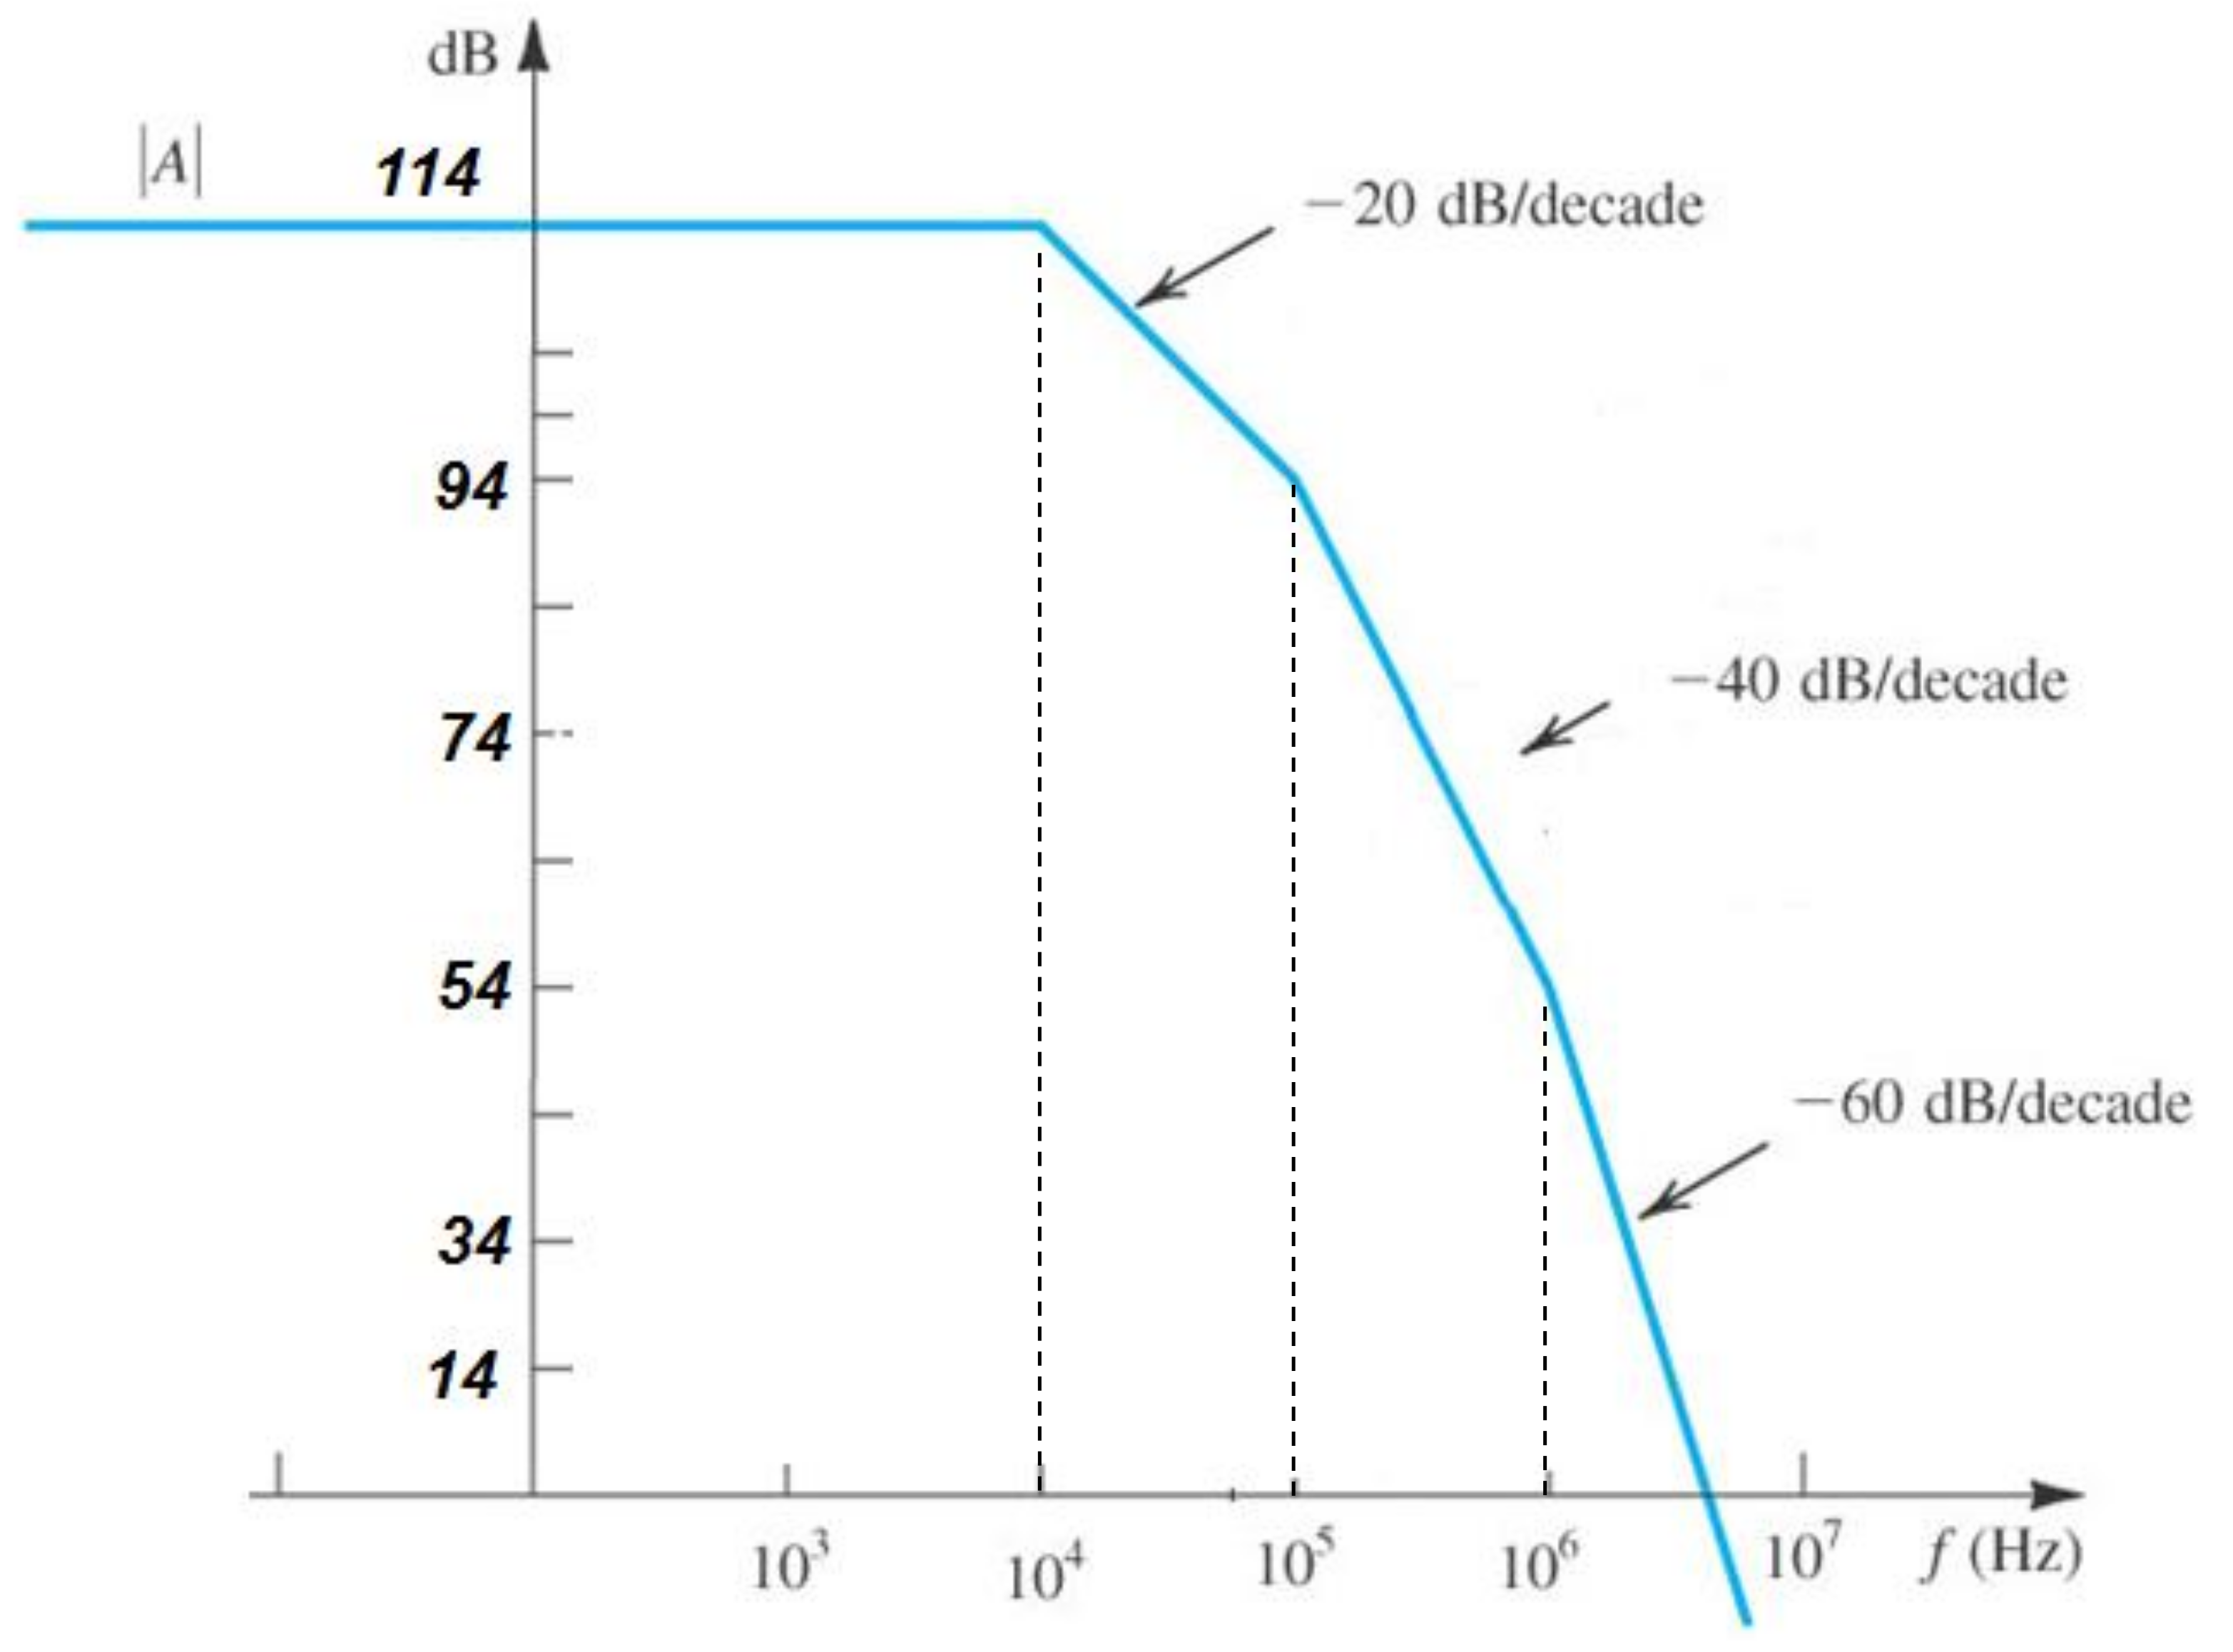
\includegraphics[width=0.4\textwidth]{imagens/1.png}
\end{center}

\question O amplificador operacional CMOS mostrado na Figura tem SR = 60 V/$\mu s$ e largura de banda de ganho unitário ($f_t$) de 50 MHz.

\begin{parts}
 \part Calcule o valor de $V_{OV}$ para os transistores do estágio de entrada;
 \part Se a corrente de polarização do primeiro estágio é 100 $\mu A$, qual valor de $C_C$ deve ser usado?
 \part Considere um processo de fabricação do qual $\mu_p C_{OX}$ = 50 $\mu A/V^2$, qual a razão de W/L para os transistores $Q_1$ e $Q_2$?
\end{parts}

\begin{center}
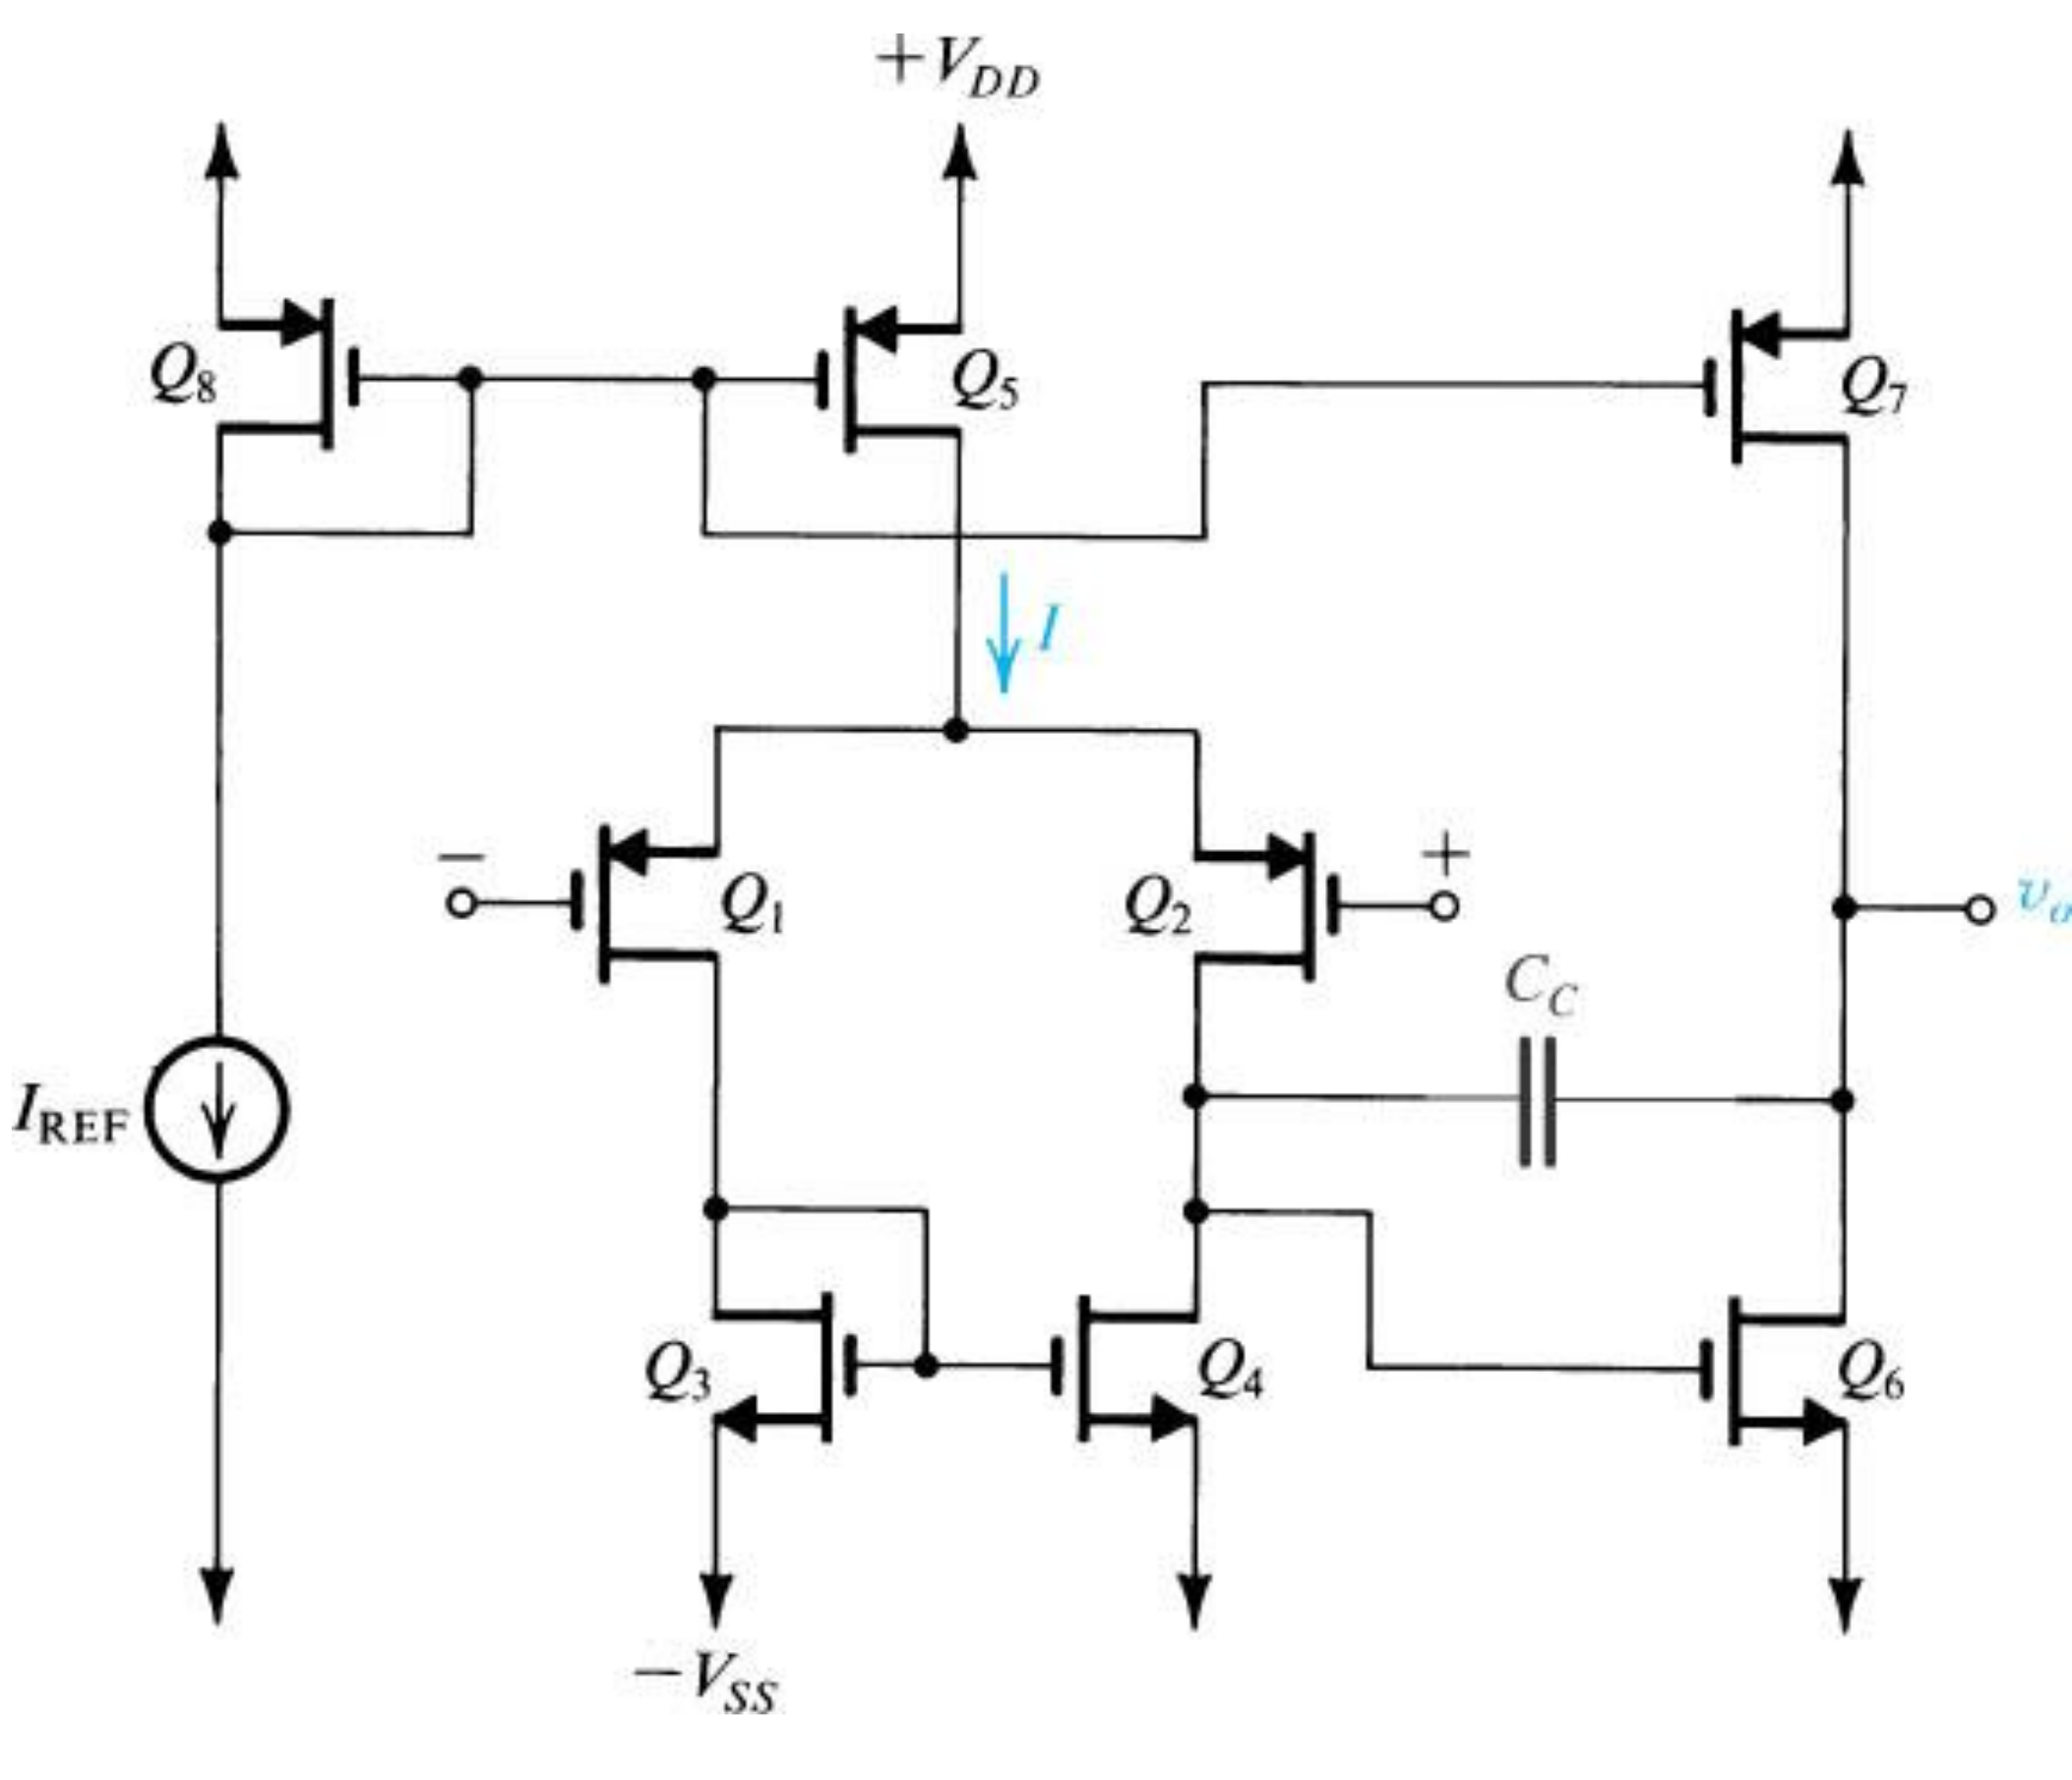
\includegraphics[width=0.4\textwidth]{imagens/2.png}
\end{center}

\question Um filtro passa-baixas do tipo Butterworth tem $A_{max} = 0,5$ dB para f $<$ $f_p$ = 1 MHz. Se a ordem do filtro não pode ser maior que 5, qual a máxima atenuação na banda de rejeição se $f_S$ = 2 MHz.

\question Dada a máscara de resposta de um filtro, determine a função de transferência de Butterwort e Chebyshev.

\begin{center}
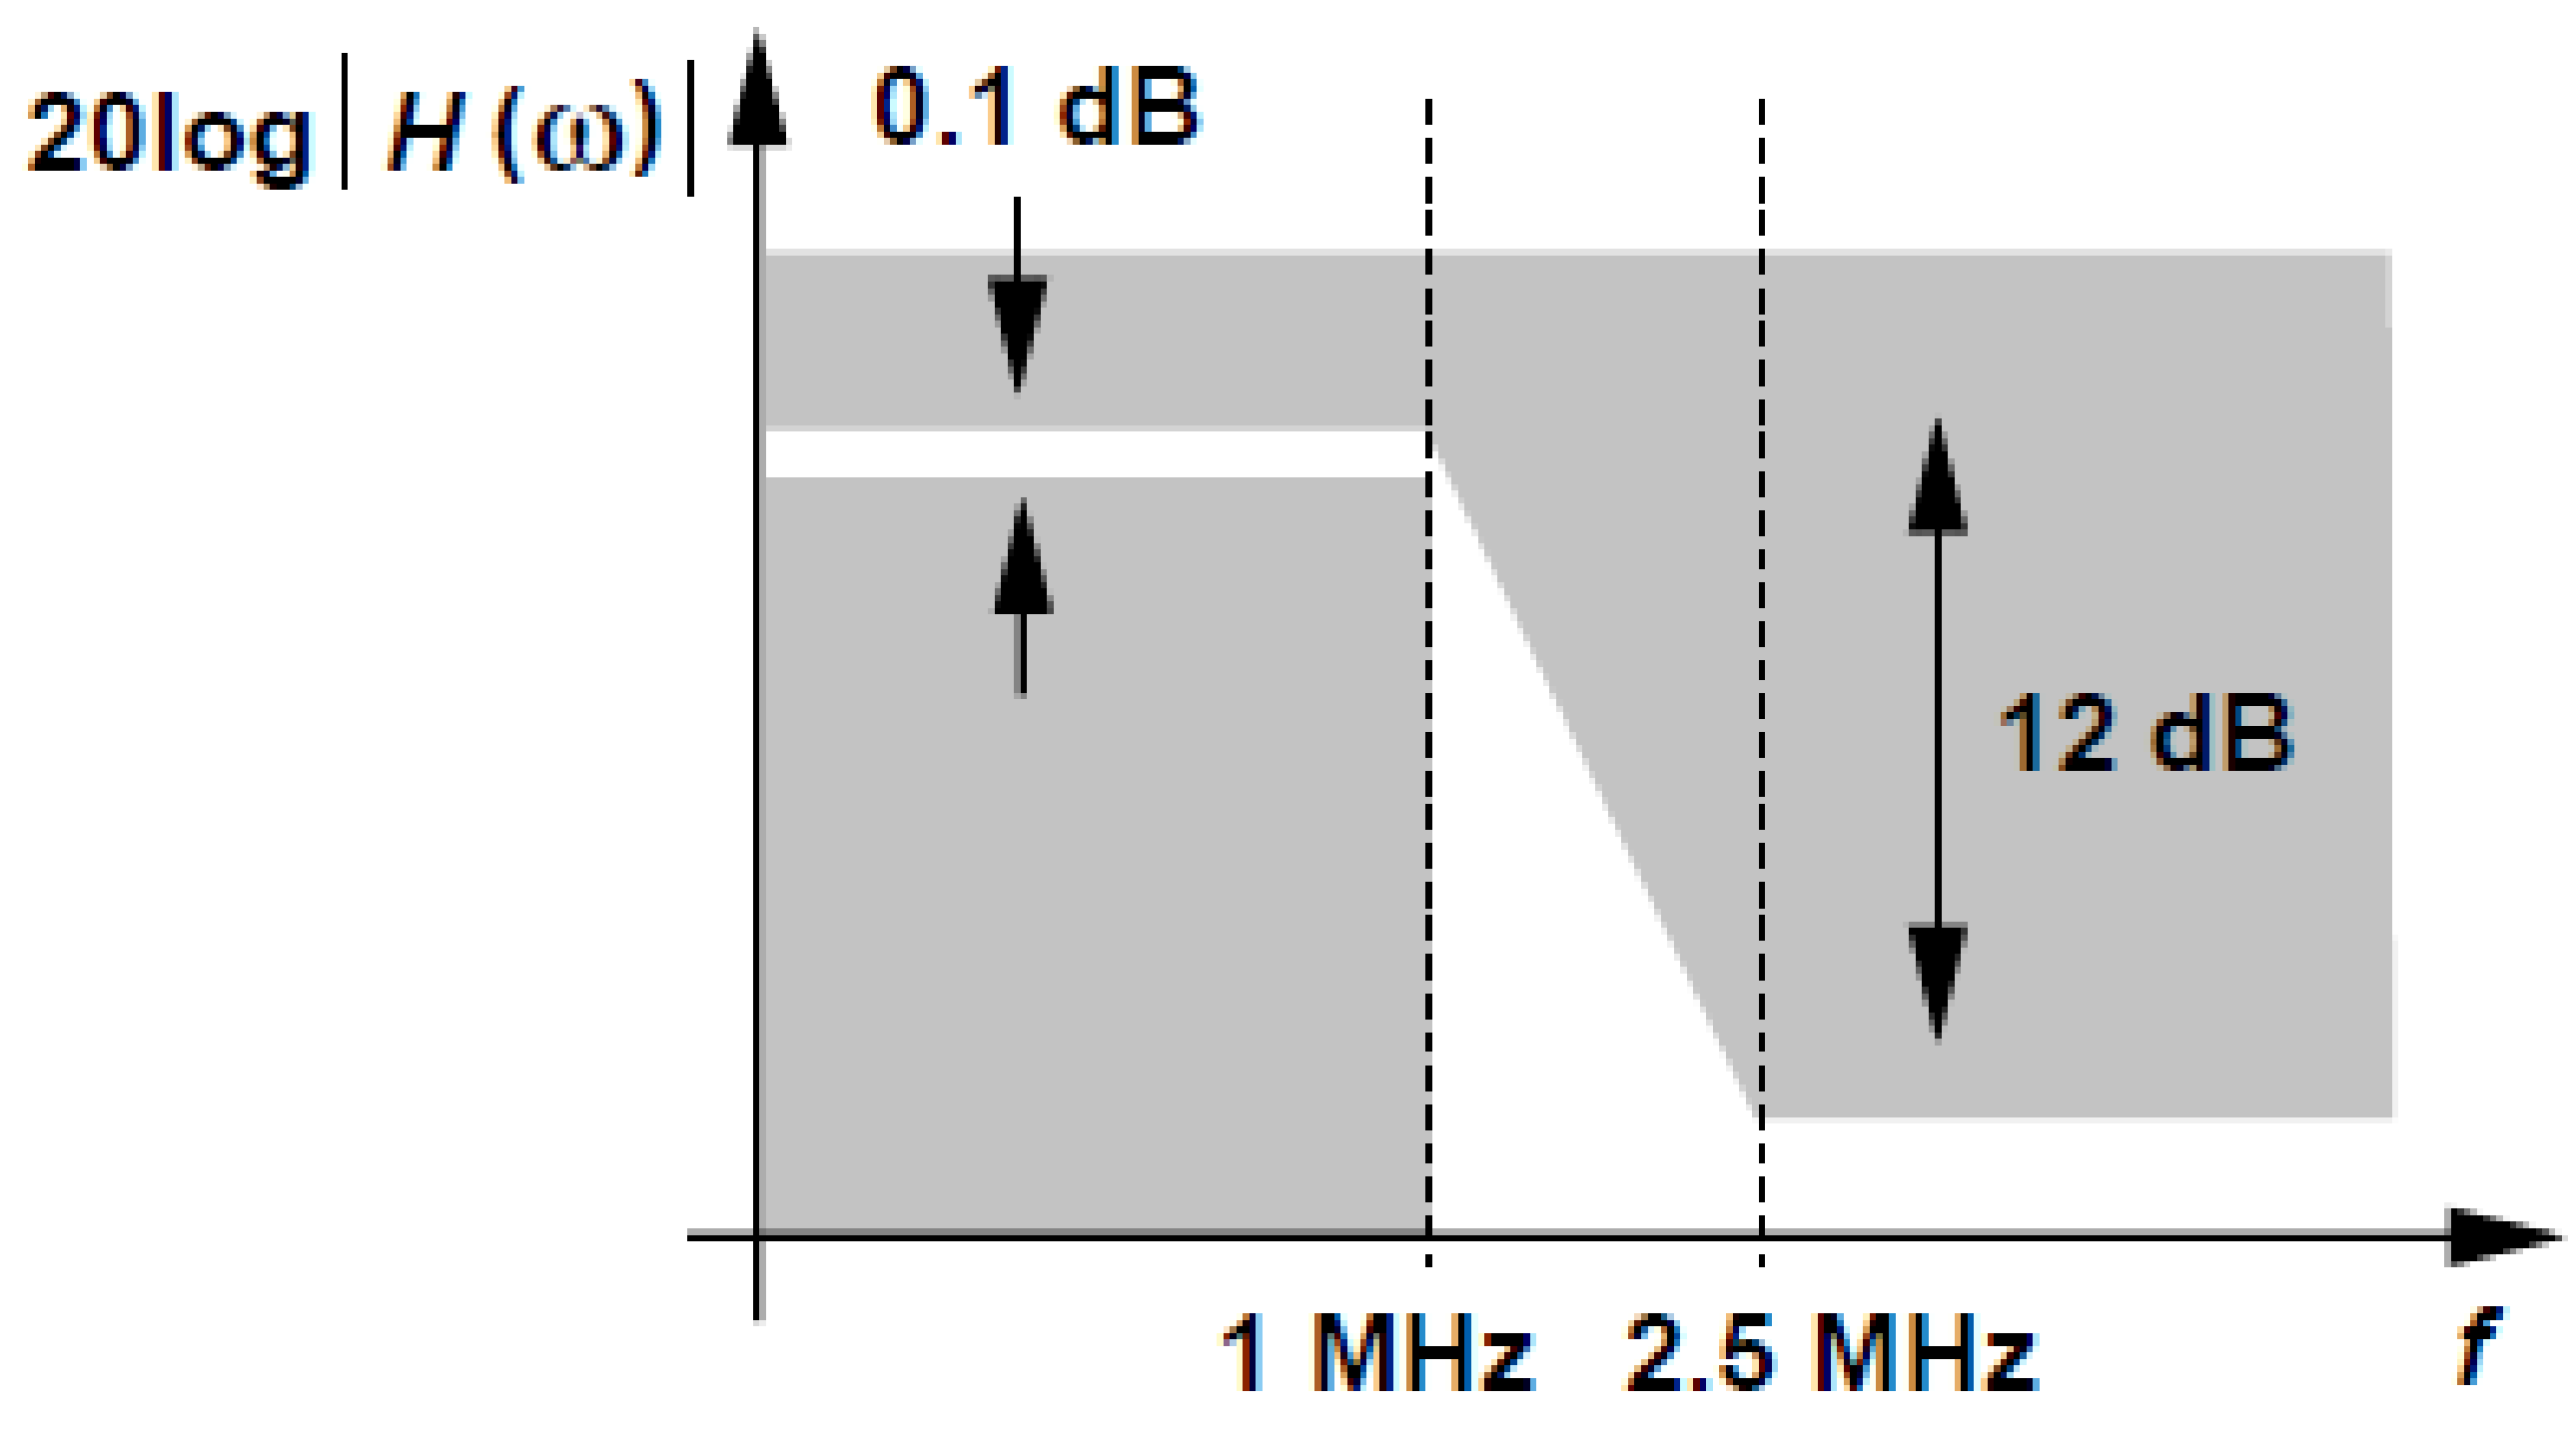
\includegraphics[width=0.4\textwidth]{imagens/3.png}
\end{center}

\question Com relação ao amplificador ua741:

\begin{parts}
 \part Como é gerada a corrente de referência?
 \part Explique como é gerado o pólo dominante neste amplificador;
 \part Apresente o diagrama em blocos e explique a função dos amplificadores de entrada, intermediário e de saída do 741.
\end{parts}

\end{questions}

\end{document}
